\documentclass[a4paper,10pt,twocolumn,uplatex,dvipdfmx]{jsarticle}

\usepackage{amsmath}
\usepackage{array}
\usepackage{booktabs}
\usepackage{graphicx}
\usepackage[alphabet]{pxchfon}
\usepackage{tabularx}
\usepackage{pdflscape}
\usepackage{capt-of}
\usepackage{xcolor}
\usepackage{url}

\setlength{\columnsep}{8mm}
\setlength{\parindent}{1zw}
\setlength{\parskip}{0.15\baselineskip}
\renewcommand{\arraystretch}{1.22}
\urlstyle{same}

\definecolor{deepblue}{RGB}{36,79,121}
\definecolor{softgray}{RGB}{245,246,247}
\definecolor{unknown}{RGB}{140,40,40}

\newcolumntype{Y}{>{\raggedright\arraybackslash}X}
\newcommand{\unknownmark}{\textcolor{unknown}{\textbf{?}}}
\newcommand{\species}[1]{\textit{#1}}
\newcommand{\Tpeak}{$T_{\mathrm{peak}}$}
\newcommand{\dTpeak}{$\Delta T_{\mathrm{peak}}$}

\title{\textbf{生理制約付き Retina SNN による\\
RGC 動的有効受容野モデリング}}
\author{M1 TANG YU}
\date{2026年7月30日}

\begin{document}

\maketitle

\begin{abstract}
本研究は、霊長類網膜の回路構造と生理的範囲を明示的な制約として用い、
直接測定が不足するパラメータを記録 RGC 応答から学習する
動的有効受容野モデリング手法を提案する。錐体、H1 水平細胞、
ON/OFF 双極細胞、局所アマクリン細胞、ON/OFF RGC を
解釈可能な処理段として構成し、接続方向、極性、局所性、細胞型を固定する。
結合強度、時定数、抑制動態、適応特性は生理的範囲内で学習し、
RF は学習後の RGC 応答から推定する。主評価にはマカク記録データを用い、
ヒト設定は独立した転移プロファイルとして扱う。細胞間接続、
既知・未知の生理データ、パラメータ決定方針、学習手順、
実験上のリスクと対照条件を一体として整理する。
\end{abstract}

\section{研究目的と提案手法の位置づけ}

\subsection{研究目的}

本研究の目的は、既知の霊長類網膜回路と生理的パラメータ範囲を
モデル内部へ組み込み、RGC の動的有効受容野を記録応答から同定できる
生理制約付きグレーボックス SNN を構築することである。
入力段では ISETBio により光学像と錐体励起を生成し
\cite{brainard2015}、水平細胞、双極細胞、アマクリン細胞、RGC の
各処理段を明示する。

受容野を記述する LN/GLM と point-process model は、
刺激フィルタ、発火履歴、細胞間結合を解釈可能な形で推定できる
\cite{pillow2008}。霊長類 midget 経路については、
文献由来の回路・空間パラメータを統合する信号処理モデル
\cite{somaratna2025}、光学・解剖・生理を偏心度ごとに統合する
image-computable RF mosaic
\cite{cottaris2026} が報告されている。本研究はこれらの知見を基盤とし、
明示的な中間細胞、時間動態、スパイク生成、部分学習可能な生理制約、
学習後の dynamic RF 評価を同一の枠組みで扱う。

\subsection{中心仮説}

生理制約は、自由度の高い応答近似と比較して、少数データ条件における
RF の安定性、刺激統計をまたぐ汎化、細胞型ごとの整合性、
回路機構の追跡可能性を高めると仮定する。予測性能、RF の再現性、
学習パラメータの生理範囲、機構消融の結果を組み合わせて検証する。

\subsection{回路として固定する要素}

モデルは次の生理的制約を保持する。

\begin{itemize}
  \item L/M 錐体から H1 水平細胞への入力と、H1 から錐体終末への側方フィードバック
  \item 錐体から ON/OFF 双極細胞への符号反転・符号保存分岐
  \item 双極細胞から RGC への直接興奮性経路
  \item 双極細胞からアマクリン細胞を介する並列抑制経路
  \item ON/OFF RGC と視神経スパイク出力
\end{itemize}

これらはネットワークトポロジーと符号を定める。定量値の扱いは
DATA-FIXED、BIO-FIXED、BOUNDED-LEARNED、
VALIDATION-TUNED、POST-HOC の五区分で管理する。

\section{信号フロー図とデータの構成}

図\ref{fig:retina-flow}は、自然画像から視神経出力までの回路構造を示す。
通常矢印は興奮性入力、
曲線矢印はフィードバック、T 字端は抑制、破線は弱い入力、
二重線はネットワーク結合を表す。

細胞間の収束・発散関係は表\ref{tab:connectivity}に示す。
錐体密度、受容野径、応答時間、測定条件、物種差は
表\ref{tab:physiology}に示す。これにより、回路の接続関係と
定量的な生理根拠を独立して参照できる。

\begin{figure*}[t]
  \centering
  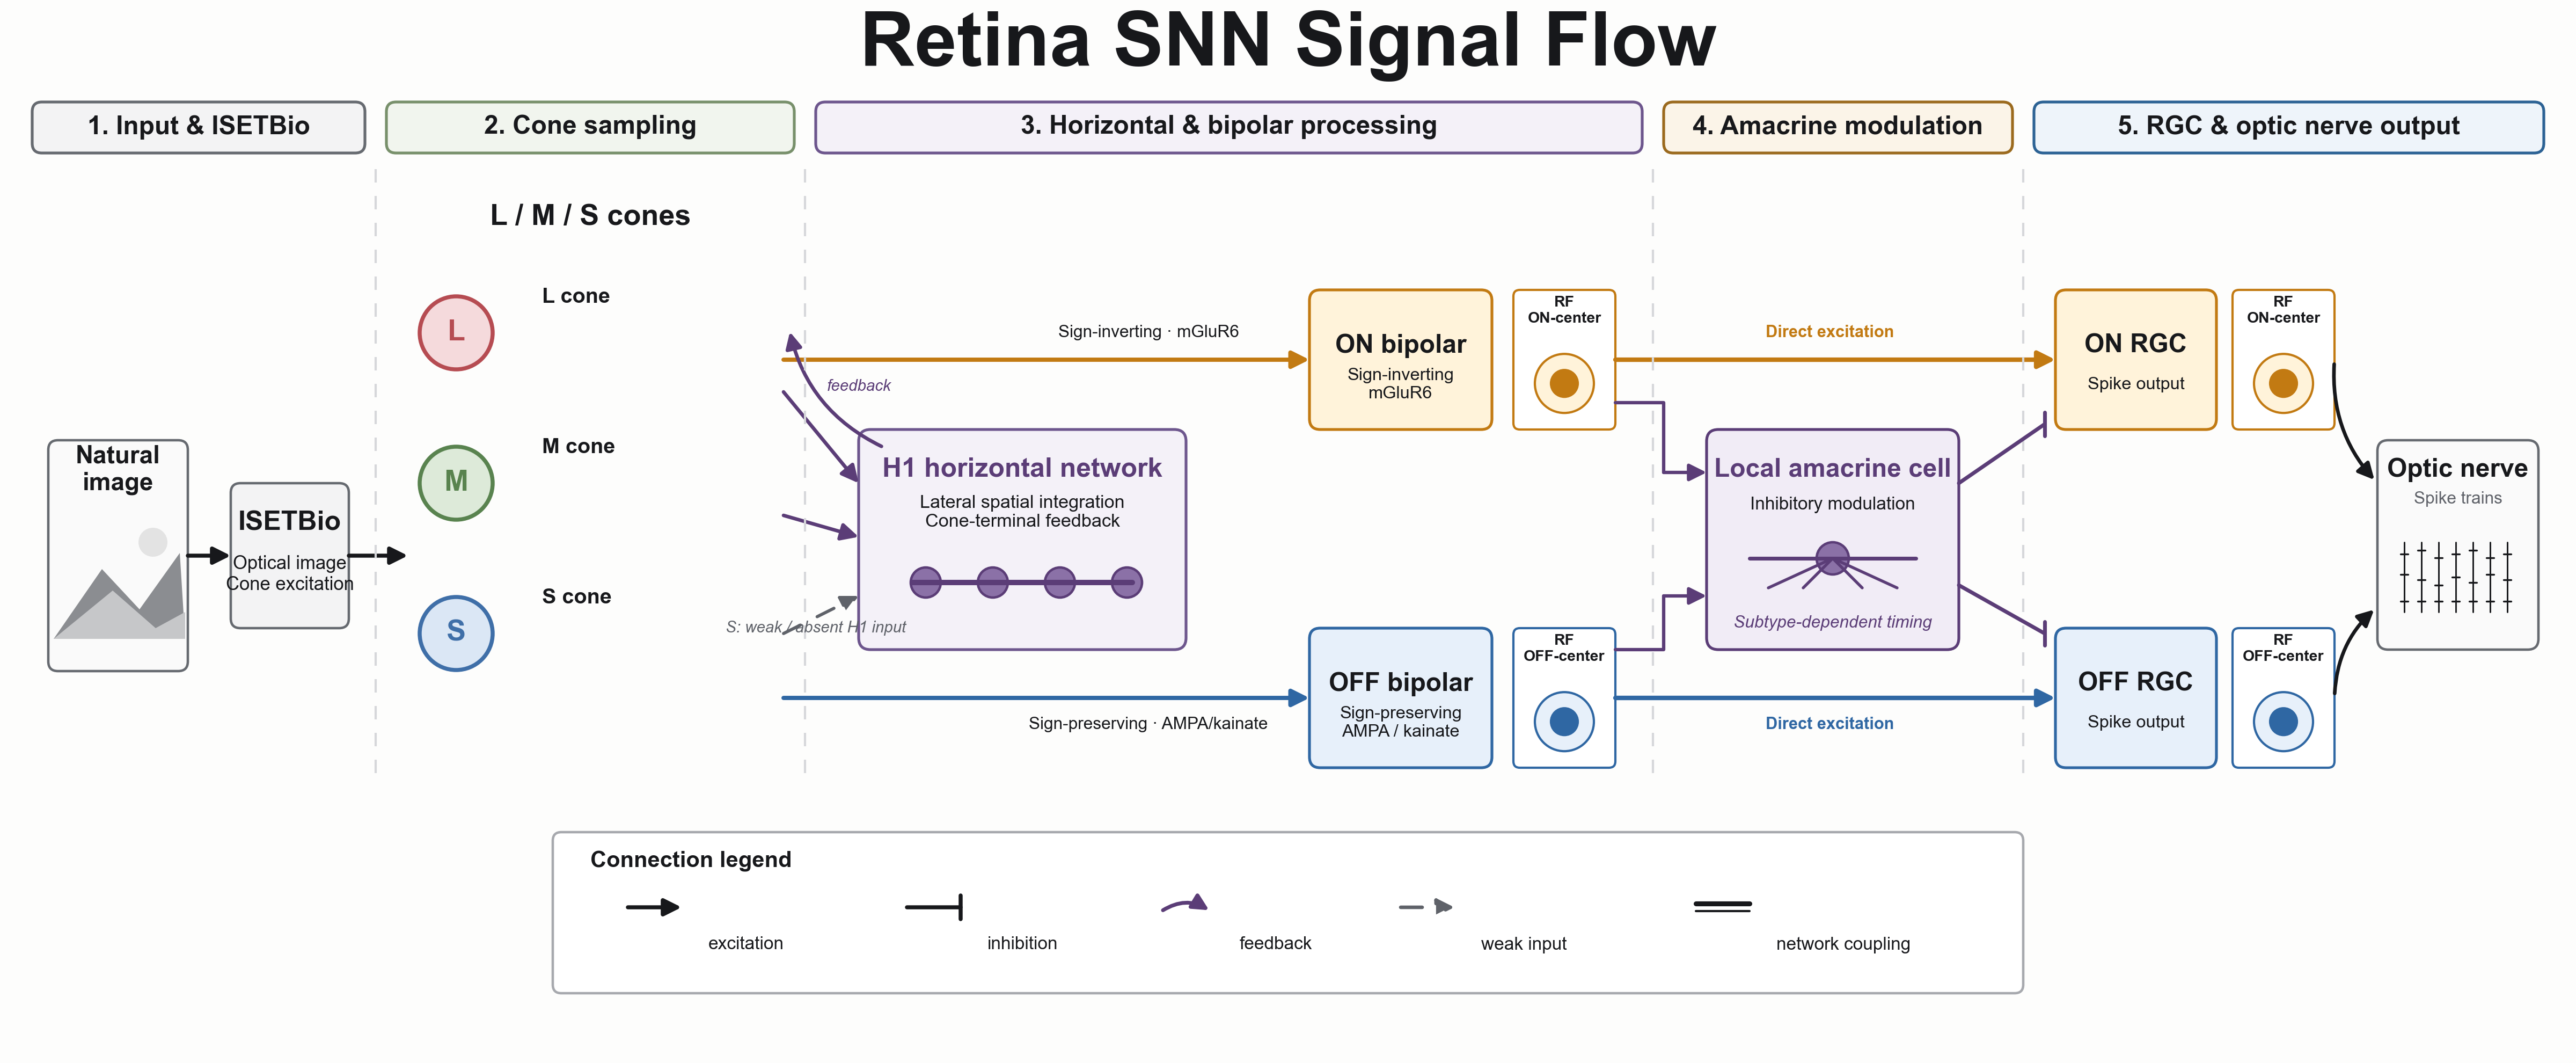
\includegraphics[width=\textwidth]{assets/retina_snn_signal_flow.png}
  \caption{Retina SNN の生理信号フロー。回路構造と接続種別を示す。
  細胞間接続は表\ref{tab:connectivity}、定量的な生理データは
  表\ref{tab:physiology}に示す。}
  \label{fig:retina-flow}
\end{figure*}

\section{信号フローの解釈}

\subsection{入力と錐体}

自然画像は ISETBio により網膜面の光学像へ変換され、
L、M、S 錐体の励起として表現される。図中の三つの錐体は
三種類の入力チャネルを表す簡略記号である。
ヒトとマカクでは錐体密度や L:M 比が同一ではないため
\cite{curcio1990,hofer2005,packer1989,munds2022}、
モデルでは物種別パラメータを明示的に切り替える必要がある。

\subsection{水平細胞と双極細胞}

マカク H1 水平細胞は主に L/M 錐体入力を受け、S 錐体入力は
弱い、または測定上認められない。一方、H2 は S 錐体入力が強い
\cite{dacey1996}。本研究の主経路は輝度処理を担う L/M--H1 系であるため、
図では H1 を主ノードとして示し、S$\rightarrow$H1 は破線で示した。

錐体終末から ON 双極細胞への伝達は mGluR6 を介する符号反転、
OFF 双極細胞への伝達は AMPA/kainate 型受容体を介する符号保存として
表現する。双極細胞の center--surround は H1 を含む外網状層回路に
依存する。H1 は狭い直接入力成分と広い coupled network 成分で表現する。

\newpage
\subsection{アマクリン細胞と RGC}

アマクリン細胞は多数のサブタイプを含む
\cite{masland2012}。現在のモデルではサブタイプが一意に確定していないため、
図では ``Local amacrine cell'' とした。双極細胞から RGC への直接経路を
主経路として残し、アマクリン細胞はそれを遮断しない並列抑制経路として示す。
したがって、アマクリン細胞に単一の普遍的な受容野径や遅延を与えることはしない。

RGC は ON-center と OFF-center に分け、軸索出力を視神経の
スパイク列として示す。midget と parasol の数値は偏心度、
測定条件、解剖学的樹状野と生理学的受容野の違いに依存するため、
表\ref{tab:physiology}で条件とともに整理する。

\clearpage
\onecolumn

\begin{landscape}
\section{細胞間の接続関係}

\captionof{table}{錐体から RGC までの分布、収束、発散、接続関係。
一つの定数で表現できない項目は \unknownmark{} とした。}
\label{tab:connectivity}

\scriptsize
\setlength{\tabcolsep}{3.5pt}
\begin{tabularx}{0.98\linewidth}{
  >{\raggedright\arraybackslash}p{0.115\linewidth}
  >{\raggedright\arraybackslash}p{0.175\linewidth}
  >{\raggedright\arraybackslash}p{0.235\linewidth}
  >{\raggedright\arraybackslash}p{0.245\linewidth}
  >{\raggedright\arraybackslash}p{0.13\linewidth}}
\toprule
\textbf{部位・物種} &
\textbf{経路} &
\textbf{分布・収束} &
\textbf{発散・下流接続} &
\textbf{証拠種別・文献} \\
\midrule

発達期ヒト中心窩 &
L/M cone $\rightarrow$ ON midget bipolar
$\rightarrow$ ON midget RGC &
serial EM connectome が受容野中心の single-cone resolution を示す。
各 ON private-line branch では cone : bipolar : RGC $=1:1:1$。 &
一つの cone は ON 系と OFF 系へ分岐する。
周辺機構には水平細胞回路が加わる。 &
解剖学・接続構造
\cite{zhang2020} \\

発達期ヒト中心窩 &
L/M cone $\rightarrow$ OFF midget bipolar
$\rightarrow$ OFF midget RGC &
OFF private-line branch も受容野中心で
cone : bipolar : RGC $=1:1:1$ の single-cone resolution を形成する。 &
ON 系と並列に構成され、同一 cone から極性別経路が生じる。 &
解剖学・接続構造
\cite{zhang2020} \\

中心窩・マカク &
L/M cone $\rightarrow$ midget bipolar
$\rightarrow$ midget RGC &
受容野中心は single-cone input を保つ。
L/M 経路で bipolar--RGC 間の興奮性シナプス数に差が報告される。 &
cone は ON/OFF midget bipolar へ分岐し、
各 branch が対応する midget RGC 中心を駆動する。 &
解剖学的データ
\cite{calkins1994} \\

中心網膜から周辺網膜・マカク &
cone / midget bipolar $\rightarrow$ midget RGC &
中心部は single-cone center。偏心度の増加に伴い、
複数の cone--midget bipolar 入力が一つの midget RGC 中心へ収束する。 &
収束数と spatial support は偏心度に依存する。
全網膜共通の固定比率は \unknownmark{}。 &
解剖学的データ + 生理測定
\cite{wool2018} \\

全網膜・マカク &
cone $\leftrightarrow$ H1/H2 horizontal cell &
水平細胞 soma は regular mosaic を形成する。
一つの cone は各型 3--5 個の水平細胞と接触するという解剖学的推定。 &
H1 は L/M 優位、H2 は S 強入力と L/M 弱入力を持つ。
network coupling と cone-terminal feedback が広い空間統合を作る。 &
解剖学的データ + マカクでの直接測定
\cite{wassle1989,dacey1996} \\

中周辺部・マカク &
cone $\rightarrow$ DB3 diffuse bipolar
$\rightarrow$ OFF parasol RGC &
一つの OFF parasol RGC に約 50 個の DB3、約 500 シナプス。
DB3 集団の上流は約 250 cone と推定される。 &
diffuse bipolar pooling が midget 系より広い
parasol center support を構成する。 &
解剖学的データ
\cite{jacoby2000} \\

未確定サブタイプ &
ON/OFF bipolar $\rightarrow$ local amacrine
$\dashv$ bipolar/RGC &
アマクリン細胞は多数のサブタイプを含み、空間範囲、
収束数、時間特性がサブタイプごとに異なる。 &
抑制性の並列経路を形成する。generic node に対応する
サブタイプ、収束比、発散比は \unknownmark{}。 &
不明（サブタイプ依存）
\cite{masland2012,protti2014} \\

\bottomrule
\end{tabularx}

\vspace{0.7\baselineskip}
\noindent\textbf{表の説明：}
中心窩の $1:1:1$ は、発達期ヒト中心窩の serial EM で示された
\textbf{各 ON/OFF private-line branch の受容野中心}を指す。
cone から ON/OFF への分岐、水平細胞を介する周辺機構、偏心度に伴う
midget 経路の収束を同時に扱う。発達段階、物種、偏心度、細胞サブタイプを
接続比のキーとする。\unknownmark{} は、generic amacrine node に
一つの細胞数比を割り当てるためのサブタイプ情報が不足していることを示す。

\end{landscape}

\clearpage
\section{パラメータ決定方針}

パラメータは由来と選定方法に基づいて五区分に分ける。

\begin{center}
\centering
\captionof{table}{パラメータ区分。}
\label{tab:parameter-class}
\small
\setlength{\tabcolsep}{5pt}
\begin{tabularx}{0.92\textwidth}{
  >{\raggedright\arraybackslash}p{0.20\textwidth}
  >{\raggedright\arraybackslash}p{0.31\textwidth}
  Y}
\toprule
\textbf{区分} & \textbf{決定原理} & \textbf{代表例} \\
\midrule
DATA-FIXED &
データファイルと実験プロトコルから決定し、学習中は固定 &
時間軸、cone/cell position、cell mapping、stimulus split \\
BIO-FIXED &
高信頼の生理・解剖知見からトポロジー、極性、順序を固定 &
ON/OFF 分岐、局所接続、興奮/抑制符号、直接 bipolar$\rightarrow$RGC 経路 \\
BOUNDED-LEARNED &
文献値から初期値、上下限、型間順序を設定し、記録応答から推定 &
時定数、gain、threshold、adaptation、local spatial weight \\
VALIDATION-TUNED &
validation set と training diagnostics により選択 &
learning rate、BPTT 長、gradient clipping、regularization weight \\
POST-HOC &
モデル凍結後に測定し、loss へ入力しない &
RF center/surround、latency、dynamicity、type asymmetry \\
\bottomrule
\end{tabularx}
\end{center}

\clearpage

\begin{landscape}
\section{既知・未知の生理データ}

\captionof{table}{Retina SNN に関係する生理・解剖データの整理。
直接比較できる値が選定できていない欄は \unknownmark{} とした。}
\label{tab:physiology}

\scriptsize
\setlength{\tabcolsep}{2.8pt}
\begin{tabularx}{0.98\linewidth}{
  >{\raggedright\arraybackslash}p{0.095\linewidth}
  >{\raggedright\arraybackslash}p{0.175\linewidth}
  >{\raggedright\arraybackslash}p{0.215\linewidth}
  >{\raggedright\arraybackslash}p{0.215\linewidth}
  >{\raggedright\arraybackslash}p{0.14\linewidth}
  >{\raggedright\arraybackslash}p{0.075\linewidth}}
\toprule
\textbf{細胞・指標} &
\textbf{ヒト} &
\textbf{マカク} &
\textbf{測定条件・定義上の注意} &
\textbf{証拠 / モデル用途} &
\textbf{文献} \\
\midrule

錐体密度 &
ピーク平均 199,000 cones/mm$^2$（100,000--324,000）、
総数平均 4.6 million（4.08--5.29 million）。 &
\species{M. nemestrina}：ピーク平均 210,000 cones/mm$^2$
（190,000--260,000）、総数平均 3.1 million（2.8--3.3 million）。 &
いずれも postmortem whole-mount anatomy。ピーク位置と個体差を伴う。 &
解剖学的データ / DATA-FIXED。物種・偏心度別の geometry prior。 &
\cite{curcio1990,packer1989} \\

L:M 比・S 錐体割合 &
L:M $=1.1:1$--$16.5:1$。
約 $1^{\circ}$ で S cone $5.72\pm0.69\%$。 &
\species{M. mulatta}：L:M $=1.03:1\pm0.02$。
S-related expression ratio $0.143:1\pm0.002$。 &
ヒトは adaptive-optics imaging + densitometry。
マカク値は foveal opsin mRNA ddPCR による expression proxy。 &
ヒトでの直接測定 + 間接測定 / species-specific prior。 &
\cite{hofer2005,munds2022} \\

錐体応答時間 &
Dim-flash \Tpeak{} $\approx20$ ms。 &
5,000 R*/cone/s：L 36.7、M 36.3、S 45.3 ms。
50,000 R*/cone/s：L 33.1、M 34.1、S 44.5 ms。 &
ヒトは in vivo paired-flash ERG とモデルによる photocurrent 推定。
マカクは単一錐体電位応答。\Tpeak{} と synaptic delay は別指標。 &
間接測定 + マカクでの直接測定 / temporal bound と POST-HOC 比較。 &
\cite{vanhateren2006,baudin2019} \\

H1 入力選択性 &
直接生理の選択値：\unknownmark{}。 &
H1 は L/M 入力、測定上 S 入力なし又は極めて弱い。
H2 は S 強入力 + L/M 弱入力。 &
マカクの生理・解剖結果。ヒト profile では cross-species prior として記録する。 &
マカクでの直接測定 / BIO-FIXED（入力選択性と符号）。 &
\cite{dacey1996} \\

H1 受容野と時間 &
生理的 RF：\unknownmark{}。
時間：\unknownmark{}。 &
combined RF diameter 122 $\mu$m（偏心度 4 mm）、
309 $\mu$m（11 mm）。H1 は cone より \dTpeak{} $\approx4$ ms 遅い。 &
in vitro macaque retina。RF は狭い直接成分 + 広い coupled 成分。
4 ms は同一研究条件内の相対 peak latency。 &
マカクでの直接測定 / spatial bound、temporal POST-HOC。 &
\cite{packer2002,smith2001} \\

Midget bipolar RF &
直接生理 RF：\unknownmark{}。
時間：\unknownmark{}。 &
center diameter 42 $\mu$m（31--51）、
surround diameter 467 $\mu$m（432--515）。
時間：\unknownmark{}。 &
peripheral in vitro macaque retina。
diameter $=2\times$ Gaussian radius。 &
不明 + マカクでの直接測定 / BOUNDED-LEARNED spatial support。 &
\cite{dacey2000} \\

Diffuse bipolar RF &
直接生理 RF：\unknownmark{}。
時間：\unknownmark{}。 &
center diameter 92 $\mu$m（74--114）、
surround diameter 743 $\mu$m（594--1048）。
時間：\unknownmark{}。 &
peripheral in vitro macaque retina。
diameter $=2\times$ Gaussian radius。 &
不明 + マカクでの直接測定 / BOUNDED-LEARNED spatial support。 &
\cite{dacey2000} \\

Cone$\rightarrow$bipolar の時間 &
直接 synaptic delay：\unknownmark{}。 &
直接 synaptic delay：\unknownmark{}。 &
ON/OFF の受容体機構は既知でも、図の各層へ一律に与えられる
比較可能な delay 値は選定していない。 &
不明 / polarity BIO-FIXED、時間特性 BOUNDED-LEARNED。 &
--- \\

Generic local amacrine &
RF：\unknownmark{}、delay：\unknownmark{}。 &
RF：\unknownmark{}、delay：\unknownmark{}。 &
サブタイプ、刺激、順応状態、記録法に依存する。
generic node にはサブタイプ共通値を設定しない。 &
不明 / inhibitory sign BIO-FIXED、動態 BOUNDED-LEARNED。 &
\cite{masland2012,protti2014} \\

Midget / parasol RGC &
解剖学的 dendritic-field diameter：
$D_{\mathrm{midget}}=8.64E^{1.04}$、
$D_{\mathrm{parasol}}=70.2E^{0.65}$。
生理 RF・応答時間：\unknownmark{}。 &
P/M の center と surround は偏心度とともに増大し、
M center radius は近傍 P の約 2 倍。 &
ヒト式は $D$：$\mu$m、$E$：mm で、temporal/superior/inferior retina の
形態データ。マカク値は生理測定。 &
解剖学的データ + マカクでの直接測定 / spatial prior と POST-HOC RF。 &
\cite{dacey1992,croner1995} \\

Midget RGC 時間 &
\unknownmark{}。 &
STA \Tpeak{}：foveal $67\pm6$ ms、
central $53\pm6$ ms、peripheral $37\pm4$ ms。 &
ex vivo macaque retina。刺激・STA 定義に依存し、
錐体 \Tpeak{} や synaptic delay と直接加算しない。 &
マカクでの直接測定 / POST-HOC temporal RF。 &
\cite{sinha2017} \\

ON/OFF parasol 非対称性 &
\unknownmark{}。 &
ON RF diameter は OFF より約 20\% 大きい。
ON の peak/trough/zero-crossing 時間は OFF より 10--20\% 短い。 &
in vitro white-noise response。相対差として用いる。 &
マカクでの直接測定（機能的分類）/ POST-HOC asymmetry。 &
\cite{chichilnisky2002} \\

\bottomrule
\end{tabularx}

\vspace{0.7\baselineskip}
\noindent\textbf{表の説明：}
\unknownmark{} は、選定した一次文献の範囲で、
同じ細胞サブタイプ、偏心度、刺激、順応状態、測定定義を満たす
直接比較可能な値を確定していないことを示す。
物種間の値は source species を保持した proxy として管理する。
\Tpeak{}、\dTpeak{}、時定数 $\tau$、直接 synaptic delay は
別々のフィールドに保存する。ヒト RGC の式は解剖学的樹状野として管理する。
証拠種別は、測定対象と測定方法が直接分かる日本語で記載する。

\end{landscape}

\clearpage
\onecolumn

\section{対象物種と学習データ}

\subsection{物種プロファイル}

方法評価の主設定にはマカクを用いる。マカクでは RGC の記録応答、
受容野、時間特性、内網膜回路に関する直接生理データが比較的豊富であり、
記録 spike とモデル unit を対応させた system identification が可能である。
ヒト設定は ISETBio optics、ヒト cone geometry、ヒト解剖データを持つ
独立プロファイルとして構築し、マカクで学習した type-level dynamics を
弱い事前分布として転移する。

\begin{center}
\centering
\captionof{table}{物種と実験条件の運用方針。}
\label{tab:species-policy}
\small
\setlength{\tabcolsep}{4pt}
\begin{tabularx}{0.98\textwidth}{
  >{\raggedright\arraybackslash}p{0.14\textwidth}
  >{\raggedright\arraybackslash}p{0.20\textwidth}
  >{\raggedright\arraybackslash}p{0.20\textwidth}
  >{\raggedright\arraybackslash}p{0.23\textwidth}
  Y}
\toprule
\textbf{設定} &
\textbf{入力と生理データ} &
\textbf{学習・評価} &
\textbf{研究上の役割} &
\textbf{主要リスク} \\
\midrule
Macaque-primary &
macaque-specific stimulus geometry、cone response、RGC spike、
cell type、polarity、eccentricity &
recorded spike likelihood、dynamic RF、mechanism ablation &
提案手法の主評価、parameter identification、baseline 比較 &
種・偏心度・in vivo/ex vivo 条件の混在 \\

Human-transfer &
human optics、human cone mosaic、human anatomy &
type-level prior の転移、RF range と挙動の確認 &
ヒト視覚への適用可能性、species transfer の評価 &
inner-retinal direct physiology と spike data の不足 \\

Cross-species pilot &
human ISETBio input と macaque physiology proxy &
pipeline check、scale sensitivity、parameter-recovery control &
実装検証と仮説形成 &
一つの生物個体・物種を表す結果として解釈できる範囲が狭い \\
\bottomrule
\end{tabularx}
\end{center}

in vivo データでは対象物種の optics を含む visual-space 座標を用いる。
ex vivo retina データでは網膜面刺激と retinal-space 座標を用いる。
二つの測定条件は独立した observation model として保存する
\cite{cottaris2026}。

\subsection{学習対象}

主学習対象は記録 RGC spike response である。データ契約は
\texttt{cone\_response [stimulus,time,cone]}、
\texttt{spike\_counts [stimulus,trial,time,cell]}、
\texttt{valid\_mask}、\texttt{time\_axis\_seconds}、
cone/cell position、cell type、ON/OFF polarity、eccentricity を保持する。
target kind に応じて Bernoulli または Poisson negative log-likelihood を用い、
cell ごとの有効サンプル数をそろえて平均する。

synthetic teacher は parameter recovery、符号回復、実装の健全性を確認する。
記録データによる held-out likelihood と RF 評価を生理的主張の判定に用いる。
future cone prediction は normative control、cone reconstruction は
information-preservation control として位置づける。RF 形状は training target
に含めず、凍結後のモデル応答から STA、Jacobian、GLM readout で推定する。

\clearpage
\onecolumn
\begin{landscape}
\section{生理証拠から実装への対応}

\captionof{table}{各モデル要素の固定項目、学習項目、決定方法
（実験 identity、入力、H1、双極細胞）。}
\label{tab:model-policy}

\scriptsize
\renewcommand{\arraystretch}{1.10}
\setlength{\tabcolsep}{2.7pt}
\begin{tabularx}{0.98\linewidth}{
  >{\raggedright\arraybackslash}p{0.13\linewidth}
  >{\raggedright\arraybackslash}p{0.20\linewidth}
  >{\raggedright\arraybackslash}p{0.16\linewidth}
  >{\raggedright\arraybackslash}p{0.28\linewidth}
  Y}
\toprule
\textbf{対象} &
\textbf{具体的内容} &
\textbf{区分} &
\textbf{固定・学習方法} &
\textbf{主な識別リスク} \\
\midrule
実験 identity &
species、eccentricity、preparation、stimulus coordinates &
DATA-FIXED &
experiment metadata から一つの profile を選択し、checkpoint に保存 &
物種・偏心度・測定条件の混在 \\

時間と alignment &
\texttt{dt}、stimulus frame、spike bin、burn-in、valid mask &
DATA-FIXED &
\texttt{time\_axis\_seconds} と記録 protocol から決定 &
時間ずれを時定数が吸収 \\

cone 入力 &
position、type、eye trace、stimulus alignment &
DATA-FIXED &
入力 HDF5 の geometry を固定し、normalization は train split で算出 &
geometry mismatch、split leakage \\

回路 topology &
cone$\leftrightarrow$H1、ON/OFF split、
bipolar$\rightarrow$RGC、bipolar$\rightarrow$AC$\dashv$RGC &
BIO-FIXED &
接続方向、興奮/抑制符号、並列経路、局所 mask を固定 &
誤った topology を gain が補償 \\

local support &
H1、bipolar、AC、RGC の接続半径と mask &
BIO-FIXED + VALIDATION-TUNED &
文献範囲内の離散候補を作り、validation で選択。
mask 内の重みを学習 &
半径と weight の非識別性 \\

H1 dynamics &
feedback gain、coupling strength、time constant &
BOUNDED-LEARNED &
L/M 優位入力と負帰還符号を固定。
profile の上下限内で gain と $\tau_H$ を学習 &
ヒト direct physiology の不足、
bipolar surround との代替 \\

Bipolar dynamics &
ON/OFF gain、threshold、rectification、
sustained/transient time scale &
BIO-FIXED + BOUNDED-LEARNED &
polarity と transient $<$ sustained の順序を固定。
gain、threshold、softness、各 $\tau$ を有界学習 &
上流・下流 time scale の相互補償 \\

\bottomrule
\end{tabularx}
\end{landscape}

\clearpage
\begin{landscape}
\subsection*{RGC・学習・評価パラメータ}

\captionof{table}{各モデル要素の固定項目、学習項目、決定方法
（アマクリン、RGC、学習、RF 評価）。}
\label{tab:model-policy-rgc}

\scriptsize
\renewcommand{\arraystretch}{1.10}
\setlength{\tabcolsep}{2.7pt}
\begin{tabularx}{0.98\linewidth}{
  >{\raggedright\arraybackslash}p{0.13\linewidth}
  >{\raggedright\arraybackslash}p{0.20\linewidth}
  >{\raggedright\arraybackslash}p{0.16\linewidth}
  >{\raggedright\arraybackslash}p{0.28\linewidth}
  Y}
\toprule
\textbf{対象} &
\textbf{具体的内容} &
\textbf{区分} &
\textbf{固定・学習方法} &
\textbf{主な識別リスク} \\
\midrule

Amacrine dynamics &
inhibitory gain、time scale、local radius、feedback target &
BIO-FIXED + BOUNDED-LEARNED &
抑制符号と並列経路を固定。
radius は離散選択、gain と $\tau_A$ は有界学習 &
subtype 未確定、複数機構の同等解 \\

RGC type prior &
ON/OFF、midget/parasol、cell identity、eccentricity &
DATA-FIXED + BIO-FIXED &
記録 metadata の type label と polarity を固定。
type-level base parameter を共有 &
type prior が RF 差を事前形成 \\

RGC learnable state &
spatial sigma、sustained mix、membrane/adaptation $\tau$、
adaptation gain、threshold、subunit time/gain &
BOUNDED-LEARNED &
type-level parameter を上下限内で学習し、
cell-specific residual を小さく正則化 &
gain、threshold、input scale の相互補償 \\

出力 likelihood &
Bernoulli/Poisson target、cell bias、observed-spike history &
DATA-FIXED + BOUNDED-LEARNED &
target kind はデータ属性で固定。
bias、history、readout weight を学習 &
readout shortcut、history leakage \\

学習制御 &
learning rate、BPTT、gradient clipping、prior weights &
VALIDATION-TUNED &
validation likelihood、gradient statistics、
state stability により選択 &
validation overfitting \\

RF 指標 &
center、surround、latency、polarity、dynamicity &
POST-HOC &
モデル凍結後に STA、Jacobian、GLM から抽出 &
刺激集合と解析法への依存 \\
\bottomrule
\end{tabularx}

\vspace{0.6\baselineskip}
\noindent\textbf{表の説明：}
学習可能量は type-level shared parameter と小さな cell-specific residual に分ける。
上下限は変換パラメータ化によって常に満たし、範囲端への集中を
parameter identifiability の警告として記録する。local support の半径は
連続重みと同時に自由化せず、文献範囲内の離散 sweep で決定する。

\end{landscape}

\clearpage
\twocolumn

\section{段階的学習方針}

\subsection{Stage 0：実験 identity の固定}

species、eccentricity、preparation、stimulus coordinate、cone geometry、
cell mapping、ON/OFF polarity、connection topology、local mask を固定する。
データ split は stimulus source 単位で分離し、normalization 統計量は
training split から計算する。

\subsection{Stage 1：出力校正}

cell baseline、output bias、readout weight を先に学習し、
各 recorded cell に予測可能な信号が存在することを確認する。
この段階では上流 dynamics と type-level physiology parameter を凍結する。

\subsection{Stage 2：RGC dynamics}

RGC membrane、adaptation、history、threshold、subunit dynamics を解放する。
同一 cell type は主要パラメータを共有し、各 cell は小さな residual のみを持つ。
prior penalty と residual penalty により自由度を制御する。

\subsection{Stage 3：上流 dynamics}

学習対象を amacrine、bipolar、H1 の順に一群ずつ追加する。
各段階で直前の checkpoint、held-out likelihood、RF、parameter range、
module ablation を比較する。追加モジュールの gain がゼロ近傍へ収束する場合、
そのモジュールは記録データから識別されていないと判定する。

\subsection{Stage 4：限定的な joint fine-tuning}

全 BOUNDED-LEARNED parameter を各 bounds 内で共同最適化する。
複数 seed の推定値、境界到達率、held-out performance、RF stability を保存する。
同等性能を持つ複数パラメータ集合が残る場合、内部機構の一意性を主張しない。

\subsection{複数刺激による識別}

\enlargethispage{2\baselineskip}
white noise は空間時間 RF、flash/step/chirp は time scale と adaptation、
natural movie は自然統計下の汎化、contrast change は gain control を拘束する。
単一刺激で得られたパラメータは、別刺激条件で再評価する。

\clearpage
\twocolumn

\section{比較実験と成功条件}

\subsection{比較モデル}

\begin{enumerate}
  \item LN / point-process GLM：標準的な解釈可能 RF baseline
  \item 同容量の無制約 NN/SNN：生理制約の寄与を測る baseline
  \item 全パラメータ固定の生理モデル：データ学習の寄与を測る baseline
  \item 生理制約付き部分学習モデル：提案手法
\end{enumerate}

GLM baseline は recorded spike に対する同一 split、同一 bin、
同一 likelihood で評価する \cite{pillow2008}。各 baseline は
readout capacity、unit 数、training budget を可能な範囲でそろえる。

\subsection{評価指標}

\begin{enumerate}
  \item held-out spike negative log-likelihood と calibration
  \item seed 間の RF center/surround、polarity、latency の安定性
  \item white noise と natural movie 間の RF 一致性
  \item contrast、luminance、stimulus statistics 変化への汎化
  \item 少数データ条件の sample efficiency
  \item learned parameter の bound occupancy と type-level reproducibility
  \item H1、bipolar、amacrine、RGC dynamics の経路特異的 ablation
\end{enumerate}

\subsection{成功条件}

提案手法は、無制約モデルに近い予測性能を保ち、RF の seed stability、
cross-stimulus generalization、生理範囲内のパラメータ、
経路特異的な消融効果を同時に示した場合に支持される。
高い spike likelihood と不安定な内部パラメータが併存する場合、
応答予測能力を報告し、機構同定の結論を保留する。

\section{未確定項目とデータ取得優先度}

\begin{enumerate}
  \item generic amacrine node に対応する subtype、抑制標的、空間範囲
  \item ヒト H1 と cone bipolar の direct physiological RF
  \item ヒト midget/parasol の physiological RF と dendritic field の対応
  \item 同一刺激・順応条件で比較できる layer-to-layer temporal metric
  \item macaque-primary dataset の cone geometry、RGC position、eccentricity alignment
  \item in vivo optics と ex vivo retinal-space stimulus の observation model
\end{enumerate}

\section{まとめ}

本研究は、霊長類網膜の接続 topology、ON/OFF polarity、局所性、
細胞型、偏心度依存性を明示し、直接測定が不足する dynamics を
生理範囲内で学習する grey-box Retina SNN を扱う。
主実験は macaque recorded RGC spike fitting、ヒト設定は独立 transfer profile
として構成する。パラメータを DATA-FIXED、BIO-FIXED、
BOUNDED-LEARNED、VALIDATION-TUNED、POST-HOC に分け、
出力校正、RGC dynamics、上流 dynamics、joint fine-tuning の順に学習する。
dynamic effective RF は学習後に抽出し、GLM、無制約モデル、
全固定モデルとの比較、複数刺激、複数 seed、機構消融により評価する。

\begin{thebibliography}{99}
\small

\bibitem{brainard2015}
D. H. Brainard, A. B. Cottaris, and B. A. Wandell,
``ISETBio: Computational tools for modeling early human vision,''
\textit{Proc. SPIE}, vol. 9395, 939504, 2015.
\url{https://doi.org/10.1117/12.2080444}

\bibitem{pillow2008}
J. W. Pillow, J. Shlens, L. Paninski, A. Sher, A. M. Litke,
E. J. Chichilnisky, and E. P. Simoncelli,
``Spatio-temporal correlations and visual signalling in a complete
neuronal population,''
\textit{Nature}, vol. 454, pp. 995--999, 2008.
\url{https://doi.org/10.1038/nature07140}

\bibitem{somaratna2025}
M. A. Somaratna and A. W. Freeman,
``The receptive field construction of midget ganglion cells in primate retina,''
\textit{J. Neurophysiol.}, vol. 133, no. 1, pp. 268--285, 2025.
\url{https://doi.org/10.1152/jn.00302.2024}

\bibitem{cottaris2026}
N. P. Cottaris, B. A. Wandell, and D. H. Brainard,
``An image-computable spatio-chromatic receptive field model of the
midget retinal ganglion cell mosaic across the retina,''
\textit{J. Comput. Neurosci.}, 2026.
\url{https://doi.org/10.1007/s10827-026-00930-z}

\bibitem{curcio1990}
C. A. Curcio, K. R. Sloan, R. E. Kalina, and A. E. Hendrickson,
``Human photoreceptor topography,''
\textit{J. Comp. Neurol.}, vol. 292, no. 4, pp. 497--523, 1990.
\url{https://doi.org/10.1002/cne.902920402}

\bibitem{hofer2005}
H. Hofer, J. Carroll, J. Neitz, M. Neitz, and D. R. Williams,
``Organization of the human trichromatic cone mosaic,''
\textit{J. Neurosci.}, vol. 25, no. 42, pp. 9669--9679, 2005.
\url{https://doi.org/10.1523/JNEUROSCI.2414-05.2005}

\bibitem{packer1989}
O. Packer, A. E. Hendrickson, and C. A. Curcio,
``Photoreceptor topography of the retina in the adult pigtail macaque
(\textit{Macaca nemestrina}),''
\textit{J. Comp. Neurol.}, vol. 288, no. 1, pp. 165--183, 1989.
\url{https://doi.org/10.1002/cne.902880113}

\bibitem{munds2022}
R. A. Munds et al.,
``Variation and heritability of retinal cone ratios in a free-ranging
population of rhesus macaques,''
\textit{Evolution}, vol. 76, no. 8, pp. 1776--1789, 2022.
\url{https://doi.org/10.1111/evo.14552}

\bibitem{vanhateren2006}
J. H. van Hateren and T. D. Lamb,
``The photocurrent response of human cones is fast and monophasic,''
\textit{BMC Neurosci.}, vol. 7, article 34, 2006.
\url{https://doi.org/10.1186/1471-2202-7-34}

\bibitem{baudin2019}
J. Baudin, J. M. Angueyra, R. Sinha, and F. Rieke,
``S-cone photoreceptors in the primate retina are functionally distinct
from L and M cones,''
\textit{eLife}, vol. 8, e39166, 2019.
\url{https://doi.org/10.7554/eLife.39166}

\bibitem{wassle1989}
H. W\"assle, B. B. Boycott, and J. R\"ohrenbeck,
``Horizontal cells in the monkey retina: Cone connections and dendritic network,''
\textit{Eur. J. Neurosci.}, vol. 1, no. 5, pp. 421--435, 1989.
\url{https://doi.org/10.1111/j.1460-9568.1989.tb00350.x}

\bibitem{dacey1996}
D. M. Dacey, B. B. Lee, D. K. Stafford, J. Pokorny, and V. C. Smith,
``Horizontal cells of the primate retina: Cone specificity without spectral opponency,''
\textit{Science}, vol. 271, no. 5249, pp. 656--659, 1996.
\url{https://doi.org/10.1126/science.271.5249.656}

\bibitem{packer2002}
O. S. Packer and D. M. Dacey,
``Receptive field structure of H1 horizontal cells in macaque monkey retina,''
\textit{J. Vis.}, vol. 2, no. 4, pp. 272--292, 2002.
\url{https://doi.org/10.1167/2.4.1}

\bibitem{smith2001}
V. C. Smith, J. Pokorny, B. B. Lee, and D. M. Dacey,
``Primate horizontal cell dynamics: An analysis of sensitivity regulation
in the outer retina,''
\textit{J. Neurophysiol.}, vol. 85, no. 2, pp. 545--558, 2001.
\url{https://doi.org/10.1152/jn.2001.85.2.545}

\bibitem{dacey2000}
D. Dacey, O. S. Packer, L. Diller, D. Brainard, B. Peterson, and B. Lee,
``Center surround receptive field structure of cone bipolar cells in primate retina,''
\textit{Vision Res.}, vol. 40, pp. 1801--1811, 2000.
\url{https://doi.org/10.1016/S0042-6989(00)00039-0}

\bibitem{zhang2020}
C. Zhang, Y. J. Kim, A. R. Silverstein, A. Hoshino, T. A. Reh,
D. M. Dacey, and R. O. Wong,
``Circuit reorganization shapes the developing human foveal midget
connectome toward single-cone resolution,''
\textit{Neuron}, vol. 108, no. 5, pp. 905--918.e3, 2020.
\url{https://doi.org/10.1016/j.neuron.2020.09.014}

\bibitem{calkins1994}
D. J. Calkins, S. J. Schein, Y. Tsukamoto, and P. Sterling,
``M and L cones in macaque fovea connect to midget ganglion cells by
different numbers of excitatory synapses,''
\textit{Nature}, vol. 371, pp. 70--72, 1994.
\url{https://doi.org/10.1038/371070a0}

\bibitem{wool2018}
L. E. Wool et al.,
``Nonselective wiring accounts for red-green opponency in midget ganglion
cells of the primate retina,''
\textit{J. Neurosci.}, vol. 38, no. 6, pp. 1520--1540, 2018.
\url{https://doi.org/10.1523/JNEUROSCI.1688-17.2017}

\bibitem{jacoby2000}
R. A. Jacoby, A. F. Wiechmann, S. G. Amara, R. M. Leighton, and D. W. Marshak,
``Diffuse bipolar cells provide input to OFF parasol ganglion cells in the
macaque retina,''
\textit{J. Comp. Neurol.}, vol. 416, no. 1, pp. 6--18, 2000.
\url{https://pubmed.ncbi.nlm.nih.gov/10578099/}

\bibitem{masland2012}
R. H. Masland,
``The neuronal organization of the retina,''
\textit{Neuron}, vol. 76, no. 2, pp. 266--280, 2012.
\url{https://doi.org/10.1016/j.neuron.2012.10.002}

\bibitem{protti2014}
D. A. Protti, S. Di Marco, J. Y. Huang, C. R. Vonhoff,
V. A. Nguyen, and S. G. Solomon,
``Inner retinal inhibition shapes the receptive field of retinal ganglion
cells in primate,''
\textit{J. Physiol.}, vol. 592, no. 1, pp. 49--65, 2014.
\url{https://doi.org/10.1113/jphysiol.2013.257352}

\bibitem{dacey1992}
D. M. Dacey and M. R. Petersen,
``Dendritic field size and morphology of midget and parasol ganglion cells
of the human retina,''
\textit{Proc. Natl. Acad. Sci. USA}, vol. 89, no. 20, pp. 9666--9670, 1992.
\url{https://doi.org/10.1073/pnas.89.20.9666}

\bibitem{croner1995}
L. J. Croner and E. Kaplan,
``Receptive fields of P and M ganglion cells across the primate retina,''
\textit{Vision Res.}, vol. 35, no. 1, pp. 7--24, 1995.
\url{https://doi.org/10.1016/0042-6989(94)E0066-T}

\bibitem{sinha2017}
R. Sinha, M. Hoon, J. Baudin, H. Okawa, R. O. Wong, and F. Rieke,
``Cellular and circuit mechanisms shaping the perceptual properties of the
primate fovea,''
\textit{Cell}, vol. 168, no. 3, pp. 413--426.e12, 2017.
\url{https://doi.org/10.1016/j.cell.2017.01.005}

\bibitem{chichilnisky2002}
E. J. Chichilnisky and R. S. Kalmar,
``Functional asymmetries in ON and OFF ganglion cells of primate retina,''
\textit{J. Neurosci.}, vol. 22, no. 7, pp. 2737--2747, 2002.
\url{https://doi.org/10.1523/JNEUROSCI.22-07-02737.2002}

\end{thebibliography}

\end{document}
